\chapter{Wing Box model}
\label{chap:model}

\section{Introduction} \label{sec:introInModel}

% Introduction to the chapter

\section{Concept} \label{sec:conceptInModel}

% Explanation of the concept
% -> Bending-twist coupling
% -> Shiftable shear centre location
% -> A web with variable-stiffness capability

% Figure: Fig. 1 Raither ?, Geometry and system of coordinates.
% Figure: Fig. 2 Raither ?, Schematic of the working principle.

% -> Buckling phenomena
% Figure: Schematic representation buckling phenomena

\section{Analytical model} \label{sec:analyticalModel}

%% Analytical apprach description
% An analytical model of the Wing Box will be build.
% The twist of the beam will be calculated
%
%Figure of analytical model
\begin{figure}
  \centering
  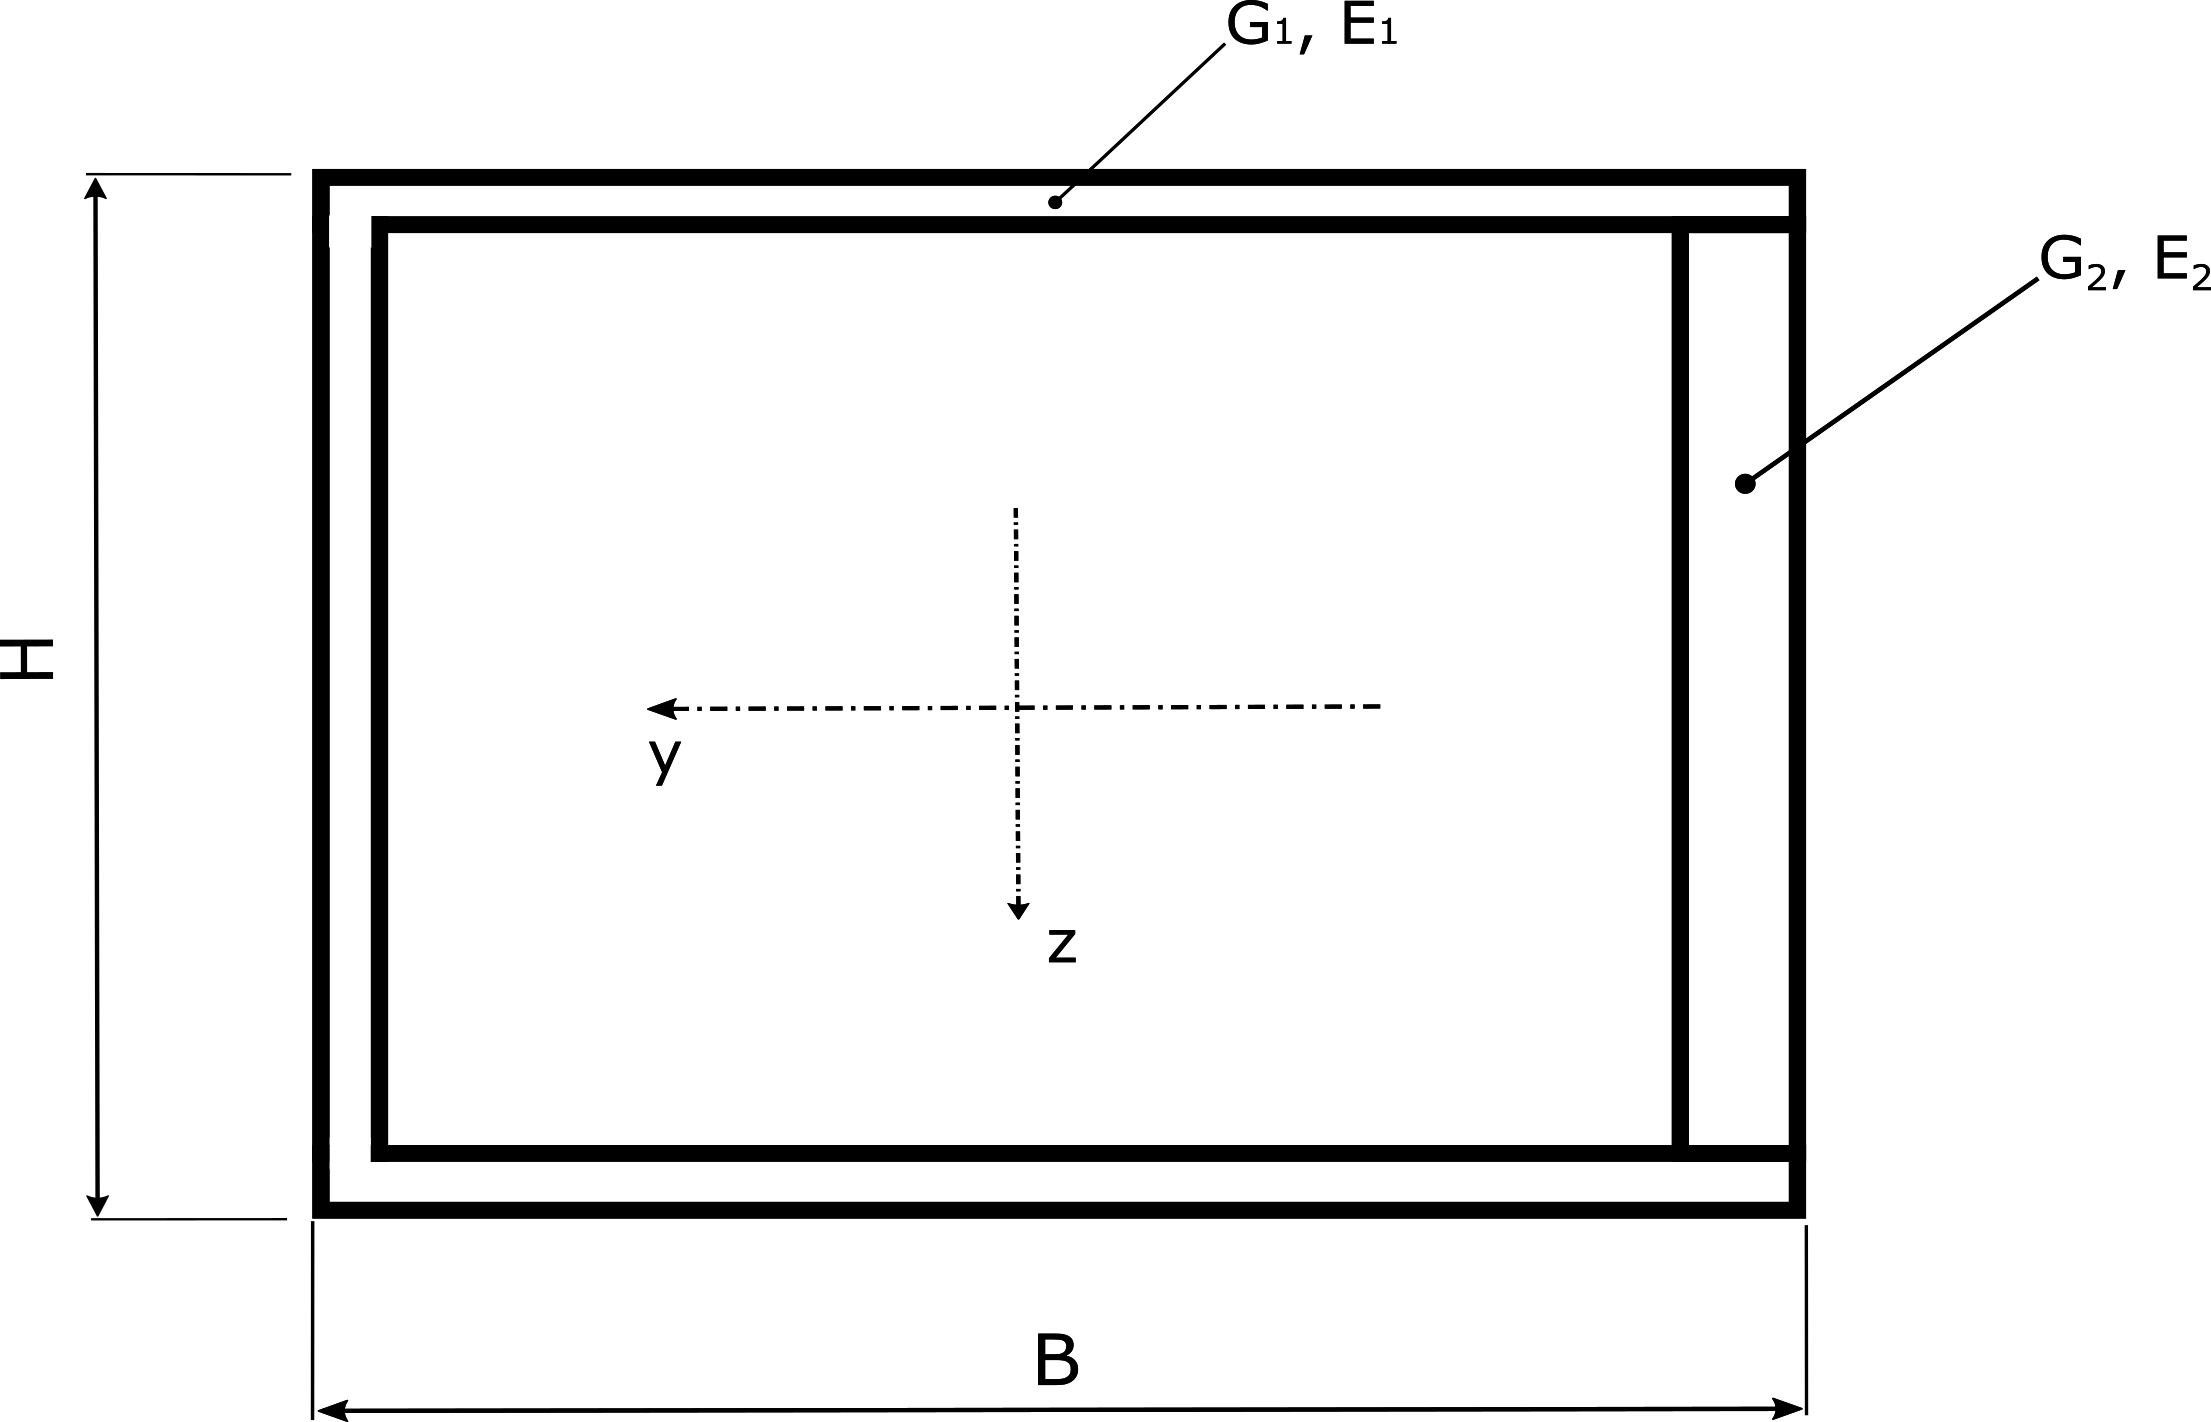
\includegraphics[width=0.8 \textwidth]{model/analyticalBox}
  \caption[Schematic view of the beam closed section]{Schematic view of the beam closed section. The dimensions are given by the width $B$ and the height $H$. For the upper, lower and left elements, the shear modulus and the elastic modulus are given by $G_1$ and $E_1$, respectively. For the right element, the same mechanical properties are given by $G_2$ and $E_2$.}\label{fig:analyticalBox}
\end{figure}

%Torsional stiffness

\begin{equation}\label{eq:torStiff}
  G I_t = \frac{4 A_0^2}{\oint \frac{\mathrm{d} s}{G(s) t(s)}}
\end{equation}

%Equations for the static moment and the flexural stiffness along the $y$ axis $\Phi_y$ (3.17, 3.18, 3.19)

%Equations for the shear flow calculation (3.20, 3.21)

%Shear centre expressions (3.22)

%The shear force is moved to the shear centre, causing an additional torsional moment given by Equation \ref{eq:momentDueToQz}. This produces a constant shear flow $q_M$ that is calculated as shown in Equation \ref{eq:constantShearFlow}.

\begin{equation}\label{eq:momentDueToQz}
  M_\mathrm{t} = Q_\mathrm{z} (y_{\mathrm{Q}} - y_\mathrm{SC})
\end{equation}
%
\begin{equation}\label{eq:constantShearFlow}
  q_M = \frac{M_\mathrm{t}}{2 A_0}
\end{equation}
%
where it has been taken into a account that a positive moment along the $x$ axis produces a constant shear flow distribution which has opposite sign as the shear flow distribution defined positive.

Finally, the total shear flow is given by the Expression \ref{eq:totalShearFlow}.

\begin{equation}\label{eq:totalShearFlow}
  q(s) = q_\mathrm{C}(s) - q_\mathrm{M}
\end{equation}

\subsection{Parametric study} \label{subsec:parametricStudy}

%Figure of analytical model
\begin{figure}
  \centering
  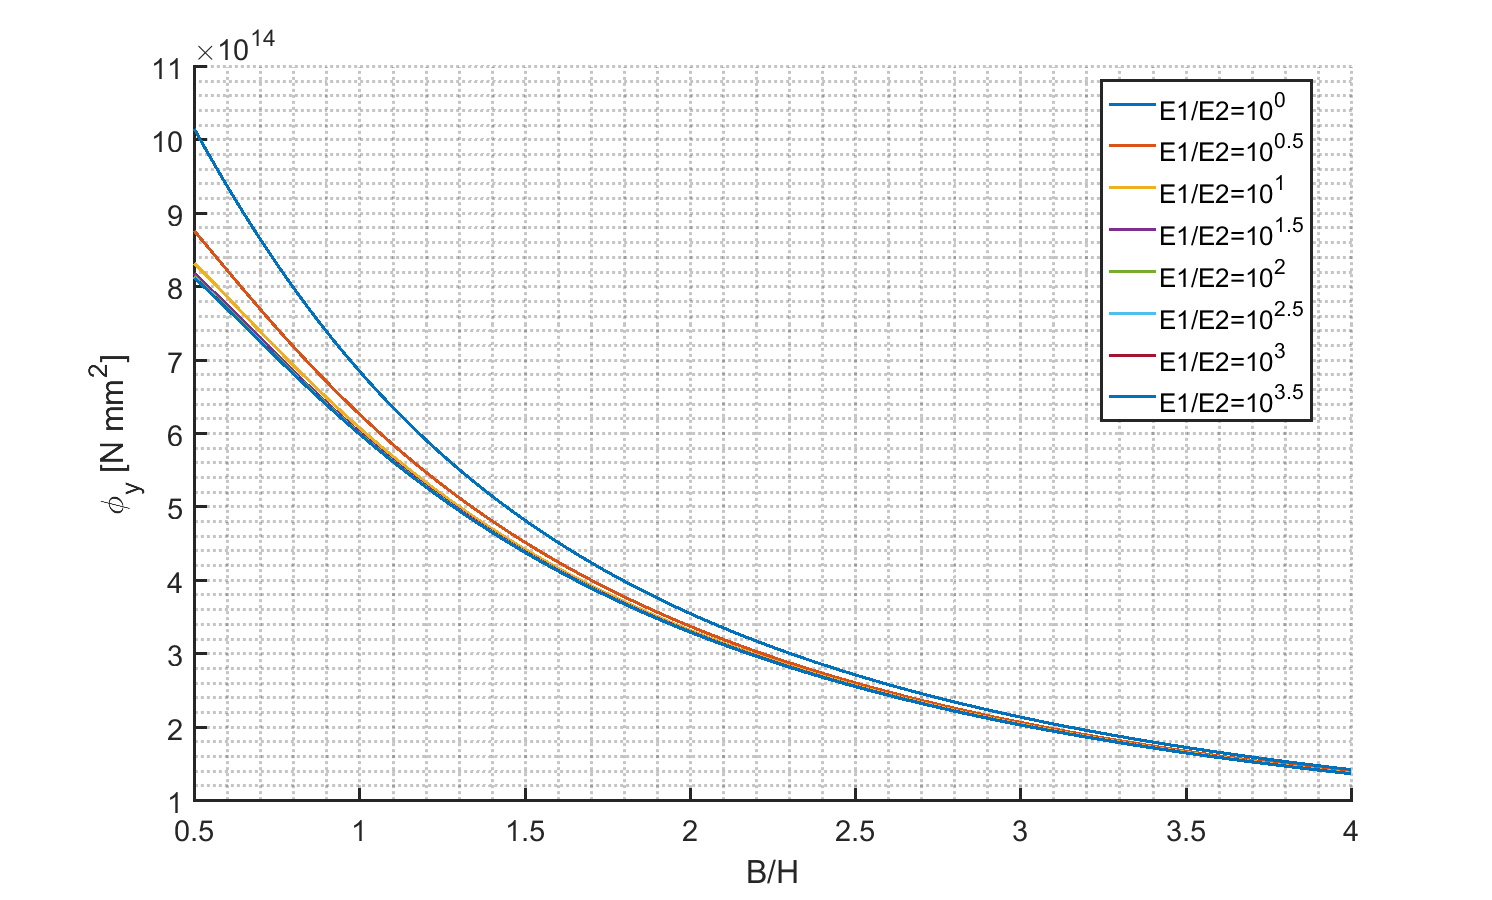
\includegraphics[width=0.8 \textwidth]{../../analytical/figures/EIy-E1overE2-BoverH}
  \caption[Blabla]{Blabla.}\label{fig:EIy_E1overE2_BoverH}
\end{figure}

\section{Computational model} \label{sec:computationalModel}

% Description of the model
%   Include all the parts of the model: C-box shape, inner box, chiral lattice
%   Figure of the model
% Parameters included
% 